\chapter{Entanglement generation in front of a static shield}\label{cha:entanglement-generation}

The generalized form of the system described in \cref{cha:first-look} with the addition of a conducting Faraday shield is shown in \cref{fig:4:complete-setup}. As before, the masses are delocalized with superposition separations $\Delta x_A$ for mass $A$ and $\Delta x_B$ for mass $B$ respectively.
\begin{figure}[!htbp]
  \centering
  \def\svgwidth{\textwidth}
  \input{./../figures/problem.pdf_tex}
  \caption{Schematic depiction of a experimental setup for the detection of gravitationally induced entanglement between two masses $A$ and $B$. They are separated by a distance of $2L + \Delta L_A + \Delta L_B$ in arbitrary orientations given by the angles $\alpha$ and $\beta$ with small variations $\Delta \theta_{A(B)}$. All variations are assumed to be gaussian distributed. The masses are delocalized in a cat state with a separation $\Delta x_{A(B)}$ between the states $\psi_{A(B)}^1$ and $\psi_{A(B)}^2$. A conducting Faraday shield with thickness $d$ is placed in the center between the masses.}
  \label{fig:4:complete-setup}
\end{figure}
The superpositions are extended in arbitrary orientations $\alpha$ and $\beta$ ($\alpha, \beta \in [0, \pi)$ because of symmetry). Most notably, the orientation of $\alpha = \beta = 0$ represents the same \q{parallel configuration} as discussed earlier and I will refer to $\alpha = \beta = \pi/2$ as the \q{orthogonal configuration}.
As demonstrated earlier, if gravity is assumed to be able to mediate entanglement, the above system can generate entanglement between states $A$ and $B$ due to their gravitational interaction.
Placing a shield in the center to shield potential interactions between the masses because of various electromagnetic interactions such as Coulomb- or Casimir-forces should in theory not influence the entanglement generation. 
However, Casimir interactions between the shield and the spheres are still present at small variations as discussed in \cref{cha:casimir-effect}.
It is straight forward to convince yourself, that these interactions can only induce local phases to each of the delocalized states depending only on the shield-mass distance of set state. 
These interactions can therefore - assuming a static shield e.g. at zero temperature - not induce any entanglement at all between different masses.

For the complete picture however, one has to consider, how the entanglement is going to be measured in a real experiment.
Most likely, the density matrix of the evolved system after some time $t$ is measured by \emph{full state tomography} !!!CITATIONS!!!. Other proposals aim to measure the entanglement using a suitable witness \cite{Bose_2017,Chevalier_2020}, but the creation of such a witness requires knowledge of the specifics on the experimental realization of massive delocalized states.
In this thesis, I will focus on the most general and universally applicable case of measuring the complete density matrix of the system and checking for entanglement.
The density matrix of a 2 qubit system however consists of 16 different entries (only 9 independent \footnote{Using the known characteristics of the density matrix like hermiticity $\rho^\dagger = \rho$ and $\tr \rho = 1$, it is possible to reconstruct $\rho$ by measuring only 9 specific entries.}) and thus at least 9 measurements of the system are required for a full state tomography. However because of the statistical nature of quantum mechanics and the fact, that each measurement destroys the previously evolved state, in practice a lot more measurements are required.
One cannot be sure that the masses are placed in the exact same position each run or if the superposition is extended in precisely the same orientation over and over again. Even if it was somehow possible, to place the particles at the \textit{exact} same position each measurement, thermal vibrations of the shield, the masses or the setup still induce small deviations in the placement.
Thus, each run the entanglement of a slightly different system is measured creating effectively a result which looks like a mixed state
\begin{equation}
  \rho = \int_{-\infty}^{\infty} \dd \theta_i \frac{1}{\sqrt{2\pi}\Delta \theta_i} e^{-\theta_i^2/2(\Delta \theta_i)^2} \ketbra{\psi_\theta} .
\end{equation}
Here, $\ket{\psi_\theta}$ is the pure state of a single measurement dependent on the angular variations $\theta_i$ ($i=A,B$). These variations are assumed to be gaussian distributed around mean $0$ and standard deviation $\Delta \theta_{A,B}$.
The same argument can be made for variations in the distance, which are distributed with $\Delta L_{A,B}$ (compare with \cref{fig:4:complete-setup}).
In some cases, like for example if the plate position moves slightly, the variations are correlated and $\Delta L_A = \Delta L_B$. But in the most general case, they are assumed to be independent and follow their own probability distribution.

\begin{figure}[!htbp]
  \centering
  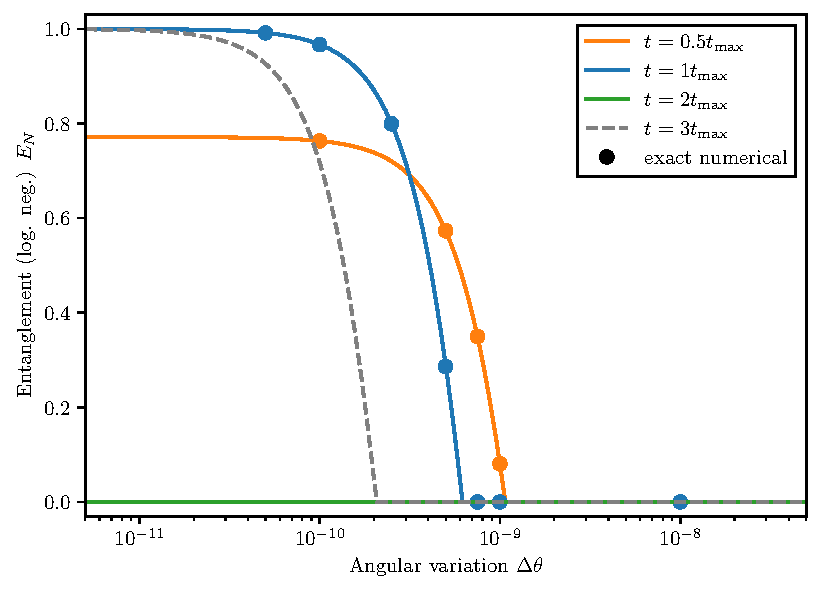
\includegraphics[width=\textwidth]{./../figures/theta-variance/EN-delta-theta.pdf}
  \caption{Entanglement quantified by the logarithmic negativity (eq. \eqref{eq:2:logarithmic-negativity}) dependent on the angular variation $\Delta\theta$. The entanglement is shown at different times, where $t_\mathrm{max}$ is the time of maximal entanglement calculable by eq. \eqref{eq:4:t-max}. Additionally, a few selected exact numerical results are shown to align precisely with the approximated version.}
  \label{fig:4:EN-delta-theta}
\end{figure}


% \section{Stability in different orientations}\label{sec:4:orientation}
As could be already seen in \cref{fig:2:entanglement-dynamics} in \cref{cha:first-look}, the entanglement dynamics and especially the time $t_\mathrm{max}$ of maximum entanglement highly depend on the orientation.
There, it was shown already, that the for the parallel configuration the maximum entanglement is reached twice as slow as in the orthogonal orientation.
This result can be more generalized for an arbitrary orientation quantified by $\alpha$ and $\beta$ from \cref{fig:4:complete-setup}.


\begin{equation}
  E_N = \log_2\left(1 + \abs{\sin\Delta \phi}\right)
\end{equation}
where $\Delta \phi$ is now dependent on the orientation and is given by (for $\Delta x \ll L$)
\begin{equation}
  \Delta \phi = \frac{G M_A M_B t}{\hbar}\frac{\Delta x_A \Delta x_B}{8 L^3} \left[\sin\alpha\sin\beta - \frac{1}{2}\cos\alpha\cos\beta\right] .
\end{equation}
The maximum entanglement is again reached after $\Delta\phi = \pi/2$ and thus is also dependent on the orientation
\begin{equation}\label{eq:4:t-max}
  t_\mathrm{max} = \frac{4\pi L^3\hbar}{GM_AM_B\Delta x_A \Delta x_B} \abs{\sin\alpha\sin\beta - \frac{1}{2}\cos\alpha\cos\beta}^{-1}.
\end{equation}
The resulting times are shown in \cref{fig:4:t-max-orientation} and align with earlier results for the special cases of the orthogonal and parallel configuration.
\begin{figure}[!htbp]
  \centering
  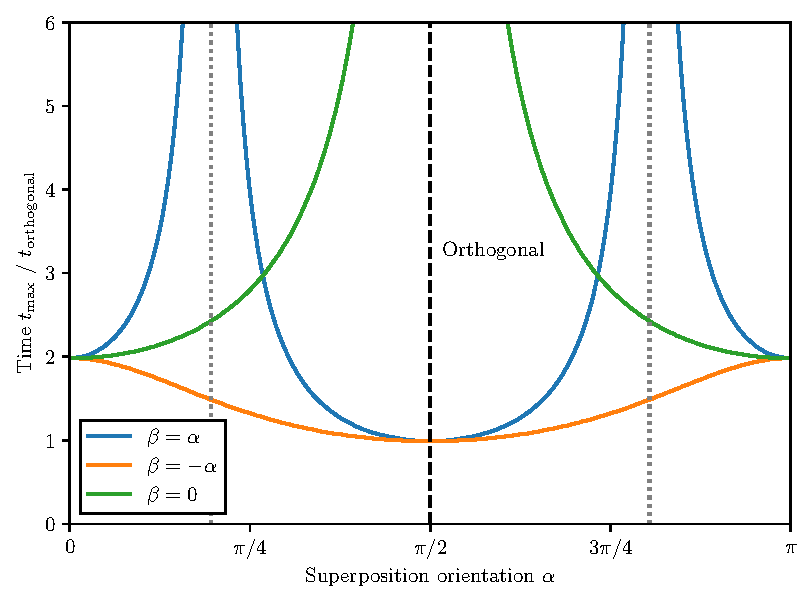
\includegraphics[width=\textwidth]{./../figures/ideal-entanglement/EN-orientation.pdf}
  \caption{Time of maximum entanglement $t_\mathrm{max}$ relative to $t_\mathrm{max,orthogonal}$ of the orthogonal configuration for different orientations. Some orientations like $\alpha=\pi/2$ and $\beta=0$ cannot induce any entanglement at all because of symmetry considerations.}
  \label{fig:4:t-max-orientation}
\end{figure}
The global minima of $t_\mathrm{max}$ is given in the orthogonal configuration meaning that of all possible configurations, this one induces entanglement the fastest. Considering the discussions in the end of \cref{cha:first-look}, this is not very surprising.
Much more interesting are the apparent singularities which arise for 
\begin{equation}
  \sin\alpha\sin\beta = \frac{1}{2}\cos\alpha\cos\beta .
\end{equation}
For $\beta=0$, the singularity in $t_\mathrm{max}$ at $\alpha=\pi/2$ is not surprising. At this configuration, the distances $\ket{\psi_A^1} \leftrightarrow \ket{\psi_B^{1,2}}$ are identical as well as $\ket{\psi_A^2} \leftrightarrow \ket{\psi_B^{1,2}}$. 
For the case $\alpha = \beta$, the two singularities are precisely given at
\begin{equation}
  \alpha = \beta = 2\arctan(\sqrt{3}\pm\sqrt{2}) \approx 90\deg \pm 54.74\deg.
\end{equation}
There does not exist a clear geometric explanation why no entanglement is generated in this configuration, however, all distances between the superpositions for a harmonic mean as visualized in \cref{fig:4:harmonic-mean}.
\begin{figure}[!htbp]
  \centering
  \def\svgwidth{\textwidth}
  \input{./../figures/harmonic-mean.pdf_tex}
  \caption{\textbf{left:} Arrangement in the orientation $\alpha=\beta=2\arctan(\sqrt{3}-\sqrt{2})$. All distances exactly lie in the \textit{harmonic mean} (for $\Delta x \ll L$). \textbf{right:} Geometric visualization of the harmonic mean.}
  \label{fig:4:harmonic-mean}
  % COLORFUL:: $\textcolor[HTML]{aa0000}{\blacksquare} = \displaystyle\frac{2}{\frac{1}{\textcolor[HTML]{0044aa}{\blacksquare}}+\frac{1}{\textcolor[HTML]{447821}{\blacksquare}}}$
\end{figure}





\begin{figure}[!htbp]
  \centering
  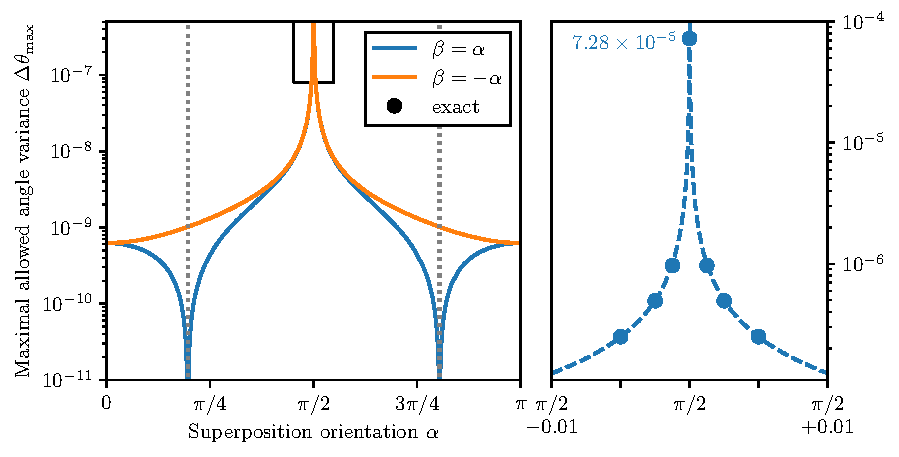
\includegraphics[width=0.95\textwidth]{./../figures/theta-variance/theta-max-orientation-complete.pdf}
  \caption{Maximum possible allowed angular variation $\Delta\theta_\mathrm{max}$ for different orientations. All data-points where calculated at the time of maximum entanglement shown in \cref{fig:4:t-max-orientation}. The \emph{orthogonal configuration} is very stable against angular disturbances. At $\alpha=\beta=\pi/2$, only exact numerical results show a finite value. The singularities on the left figure arise from the fact, that these configurations need infinite time to entangle as already seen in \cref{fig:4:t-max-orientation}.}
  \label{fig:4:theta-max-orientation}
\end{figure}

\begin{figure}[!htbp]
  \centering
  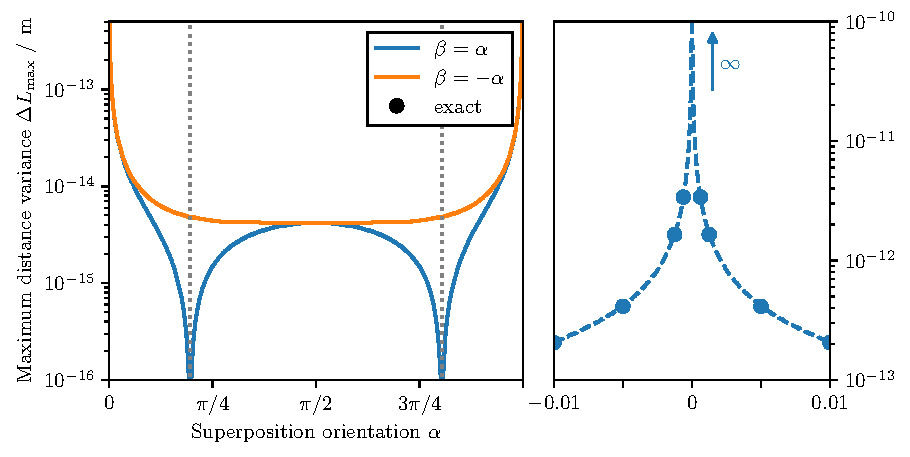
\includegraphics[width=0.95\textwidth]{./../figures/L-variance/L-max-orientation-complete.pdf}
  \caption{Maximum possible allowed distance variation $\Delta L_\mathrm{max}$ for different orientations. This figure is similar to \cref{fig:4:theta-max-orientation}, only for distance variations. On the contrary to angular variations, the \emph{parallel configuration} is infinitely stable against changes in the distance between the shield and the cat-state.}
  \label{fig:4:L-max-orientation}
\end{figure}



\begin{figure}[!htbp]
  \centering
  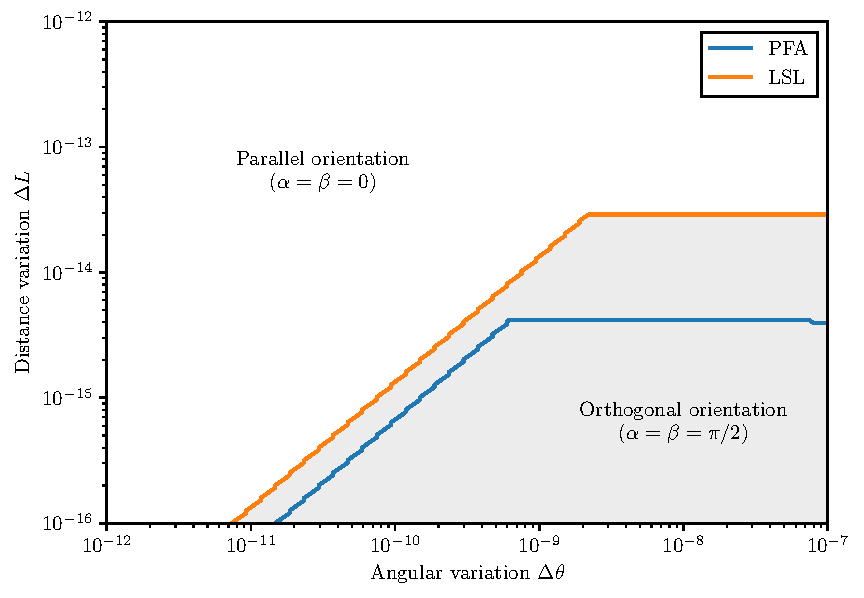
\includegraphics[width=\textwidth]{./../figures/optimize/optimized-orientation.pdf}
  \caption{Optimal orientation for arbitrary variations in the angle $\Delta\theta$ and the distance $\Delta L$. The optimum was calculated for different models of the Casimir-interaction (PFA eq. \eqref{eq:3:PFA-sphere-plate} and LSL eq. \eqref{eq:3:casimir-sphere-plate}).If angular variations dominate, the orthogonal configuration is best, whereas for large distance variations, a parallel orientation is advised.}
  \label{fig:4:optimal-orientation}
\end{figure}

\section{Discussions}\label{sec:4:discussion}
The preceding results highlight, that the proposed Faraday shield in experiments on measuring gravitationally induced entanglement entail significant engineering challenges, particularly due to the strict accuracy requirements for particle placement.
Variations must be minimized to a precision of approximately $\Delta L \simeq 10^{-10}\si{m}$ and $\Delta \theta \simeq 10^{-9}\si{rad}$, which are extremely stringent.
Even the rotation of the earth ($\omega_\mathrm{Earth}\approx 7.3\times 10^{-5}\si{rad/s}$) could potentially be problematic, because if small fluctuations in the measurement time $\Delta t \gtrsim 10^{-4}\si{s}$ are present, this corresponds to an additional angular uncertainty of $\omega_\mathrm{Earth}\Delta t \gtrsim \Delta \theta_\mathrm{crit}$.
Adjustments to the experimental parameters in \cref{tab:paramters} have to be made, where especially the separation distance $L$ and the orientation are easily changeable.

The parallel configuration is very stable against variations in the distance and might therefore be favorable (see in \cref{fig:4:optimal-orientation}).
The separation $L$ can be freely chosen and larger distances reduce the effect of placement variations as seen in \cref{fig:4:theta-crit-L}, while simultaneously increasing the required coherence time $t_\mathrm{max} \propto L^3$.

It could also be argued that at a distance of $L \geq 100\si{\mu m} = 10 R$ (compare to \cref{sec:2:experimental-problems}), the Faraday shield would no longer be required because the Casimir forces are approximately ten times weaker than gravitational interactions.
However, the loss of entanglement due to angular and distance variations is not purely due to the Casimir forces between the particle and the shield.
The gravitational coupling also depends on the placement, so that a complete removal of the shield does not fully eliminate the need for high placement accuracy.
Without the shield and by gravitational interaction alone, the critical variations are given by $\Delta \theta_\mathrm{crit,\,ideal} = 1.1 \times 10^{-3}\si{rad}$ and $\Delta L_\mathrm{crit,\,ideal} = 7\times 10^{-4}\si{m}$, which should not pose an engineering problem.

Other parameters, such as particle size and superposition size, may not be easily adjustable without increasing the complexity of quantum control.
Furthermore, particle trapping and levitation is not a limiting factor, as stable trapping is achievable for various configurations (\cref{sec:4:trapping}).

A primary aim of this thesis is to assess whether the Faraday shield allows particles to be brought closer together to enhance gravitational entanglement and reduce coherence times. 
Using the previous results, a optimal experimental parameter space can be determined.
The optimization-goal can be expressed as the following:

One wants to get \textit{as much entanglement as possible} in the \textit{shortest time possible} while allowing for the \textit{largest uncertainties} in the state preparation and considering the limitations in the particles mass as well as in the superposition size.

Without specific constraints, a general optimization is impossible because (if the mass $M$ and the superposition size $\Delta x$ is fixed) coherence time $t \propto L^3$ (eq. \eqref{eq:4:t-max}) and critical angular variation $\Delta \theta_\mathrm{crit} \propto (L-R)^3/L^3$ (for small separations) or $\Delta \theta_\mathrm{crit} \propto L^2$ (for $L \gg R$) cannot be optimized simultaneously.
With constraints such as target coherence time $t_\mathrm{target}$ and/or a minimum placement accuracy, the required sphere-plate separation $L$ as well as maximum measurable entanglement can be determined using the following steps:
\begin{enumerate}
  \item Let us assume that the size of the particle $R$ and consequently the mass $M=4/3 \pi R^3 \rho_\mathrm{Silica}$ as well as the superposition size $\Delta x$ are fixed. An increase in either of them would have a positive effect of the optimization goal stated above, as the time $t_\mathrm{max}$ decreases and the stability against placement variations increases simultaneously.
  \item Given placement accuracies in angular and separation variations determine the optimal orientation $\alpha,\beta$ of the setup as seen in \cref{fig:4:optimal-orientation}. Experimentally reachable coherence times may influence this decision slightly by taking \cref{fig:4:t-max-orientation} into account. Most likely, the most stable orientation is going to be the parallel one with $\alpha = \beta = 0$.
  \item The following ratio given by the entanglement rate eq. \eqref{eq:4:t-max}
  \begin{equation}
    \frac{M^2 (\Delta x)^2}{L^3}t_\mathrm{max} = \frac{4 \pi \hbar}{G}\abs{\sin\alpha\sin\beta-\frac{1}{2}\cos\alpha\cos\beta}^{-1} \sim 10^{-23} \si{kg^2 s/m}
  \end{equation} 
  is fixed therefore \cite{Aspelmeyer_2024}.
  \item In general it is possible to measure at an earlier time $t_\mathrm{target} = \tau t_\mathrm{max}$ (i.e. the coherence time) with $\tau \leq 1$, where less entanglement has been generated but a larger stability against placement variations can be tolerated (see \cref{fig:4:time-delta-theta}). Putting all assumptions together, the product
  \begin{equation}\label{eq:4:fixed-ratio}
    \tau L^3 = \frac{t_\mathrm{target} G M^2 (\Delta x)^2}{8\pi \hbar} = \mathrm{const.}
  \end{equation}
  of measurement time and particle-shield separation is constant.
  \item In the parallel orientation, the distance variations don't matter as the system is very stable against variations in the particle-shield separation. The critical angular variation however scales like $\Delta \theta_\mathrm{crit} \sim (L-R)^3/L^3$ for small distances and like $\Delta \theta_\mathrm{crit} \sim L^2$ at larger distances as shown in \cref{fig:4:theta-crit-L}. It is therefore possible to determine the minimum separation $L_\mathrm{min} > R$ for a given placement accuracy.
  \item Using the required separation, one can calculate $\tau \in (0, 1]$ using eq. \eqref{eq:4:fixed-ratio} and look up the maximal possible entanglement in \cref{fig:4:time-delta-theta} after an evolution time $\tau t_\mathrm{max}$.
\end{enumerate}
As an example, the radius is fixed at $R=10\si{\mu m}$ and the superposition size is $\Delta x = 100\si{nm}$. Let's say that such a particle can be placed with an accuracy of $\Delta \theta = 5 \times 10^{-8} \si{rad}$ and a coherence time of $1\si{s}$ is reachable. 
Using the steps outlined above, the required minimum particle-shield separation is around $L\approx 8R$ and the maximal amount of measurable entanglement is given by $E_N \approx 6.0\times 10^{-2}$.
For more entanglement, either a heavier particle, a larger superposition size, a higher placement accuracy or larger coherence times are required. 
It is therefore possible to bring the particles closer together than without the Faraday shield and still measure entanglement.
One is only limited by the placement accuracy and repeatability.